\chapter{算子谱}
\label{chap:operator-spectra}
\label{chap:operator-spectra-equations}

第~\ref{chap:functions-as-vectors}章把函数看成下标连成一片的无限维向量，$f$在$x$处的取值就是下标$x$上的分量。沿着这个类比，第~\ref{chap:linear-operators}章的线性算子就是无限维的矩阵：积分算子的核$k(x,y)$像矩阵元$a_{jk}$，积分$\int k(x,y)f(y)\,\mathrm dy$像求和$\sum_k a_{jk}x_k$。本章继续问矩阵论最核心的问题：一个算子能否沿某些方向简单地伸缩？

对矩阵，这个问题由特征值和奇异值回答。对称矩阵在一组标准正交基下成为对角矩阵，一般矩阵用输入、输出两组标准正交方向写成伸缩的叠加。表~\ref{tab:ospec-dictionary}列出本章要沿用的对应关系。

\begin{table}[!htb]
  \centering
  \caption{矩阵与算子的对应。左列是有限维中的已知对象，右列是函数空间中的对应物。}
  \label{tab:ospec-dictionary}
  \begin{tabular}{@{}ll@{}}
    \toprule
    矩阵 & 算子\\
    \midrule
    向量$\bm x$，分量$x_k$ & 函数$f$，分量$f(x)$\\
    矩阵$\bm A$，元素$a_{jk}$ & 积分算子，核$k(x,y)$\\
    对角矩阵$\operatorname{diag}(a_k)$ & 乘法算子$(Mf)(x)=a(x)f(x)$\\
    特征值 & 谱\\
    对称矩阵的正交对角化 & 紧自伴算子的谱分解\\
    奇异值分解 & 紧算子的奇异分解\\
    Frobenius范数 & 核的$L^2$范数\\
    \bottomrule
  \end{tabular}
\end{table}

类比有一处要特别当心。矩阵$\bm A-\lambda\bm I$不可逆时一定存在特征向量，无限维中却不然：乘以$x$的算子是一个“连续的对角矩阵”，对角元铺满整个区间，却没有一个特征函数。谱里多出来的这些点，是矩阵论中没有的现象，称为连续谱和剩余谱，第~\ref{sec:ospec-spectrum}节专门分析它们。

本章从方程$(T-\lambda I)u=g$能否对一切右端稳定求解出发，逐步加条件。第~\ref{sec:ospec-spectrum}节对一般有界算子定义谱。第~\ref{sec:ospec-compact-spectrum}节加入紧性，非零谱重新变成离散的特征值。第~\ref{sec:ospec-compact-self-adjoint}节再加入自伴性，得到正交的特征方向和展开式。

自伴性要求输入与输出在同一个空间，并排除了很多重要算子。第~\ref{sec:ospec-singular}节对两个Hilbert空间之间的一般紧算子建立奇异分解。第~\ref{sec:ospec-integral-expansion}节回到平方可积核，把这些展开写成核函数的展开，并比较核的$L^2$误差与算子范数误差。

有界性、伴随、紧性、有限秩逼近和有界逆定理都来自第~\ref{chap:linear-operators}章。谱回答的是“算子沿哪些方向怎样作用”，由输出恢复输入是否稳定，要到第~\ref{chap:linear-operator-equations}章讨论两类算子方程时才系统处理。

\section{谱}
\label{sec:ospec-spectrum}

在$n$维复空间中，$\bm A-\lambda\bm I$不可逆当且仅当它不是单射，即存在非零向量$\bm v$使$\bm A\bm v=\lambda\bm v$。有限维中单射、满射与可逆三者等价，所以“使$\bm A-\lambda\bm I$不可逆的$\lambda$”恰好就是特征值；特征值与对称矩阵的正交对角化可参考\BookChapterRef{chap:eigen-spectral-decomposition}{卷二第4章“特征值与谱分解”}。无限维中三者不再等价，算子可以是单射而不满射，因此必须直接从可逆性出发。

本节设$X\neq\{0\}$是复Banach空间，$T\in\mathcal B(X)$。要求$T$回到同一个空间，是因为$T-\lambda I$只对这样的算子有意义。实空间上的算子可以先复化：令$X_{\mathbb C}=\{x+\mathrm iy:x,y\in X\}$，按复数规则定义数乘，令$T_{\mathbb C}(x+\mathrm iy)=Tx+\mathrm iTy$；Hilbert空间中取$\lVert x+\mathrm iy\rVert^2=\lVert x\rVert^2+\lVert y\rVert^2$，它来自内积$\langle x+\mathrm iy,u+\mathrm iv\rangle=\langle x,u\rangle+\langle y,v\rangle+\mathrm i(\langle x,v\rangle-\langle y,u\rangle)$。实空间算子的谱就指$T_{\mathbb C}$的谱。

复数域是必要的。平面上旋转$90^\circ$的实矩阵$\left[\begin{smallmatrix}0&-1\\1&0\end{smallmatrix}\right]$没有实特征值，复化后才有特征值$\pm\mathrm i$。紧算子的特殊性质留到下一节，本节只讨论一般有界算子。

\subsection{谱与预解集}
\label{sec:ospec-resolvent}

参数$\lambda$“好”的含义是：对每个右端$g\in X$，方程$(T-\lambda I)u=g$都有解（存在），解只有一个（唯一），并且$g$的小误差只引起$u$的小误差（稳定）。三条合起来，就是$T-\lambda I$有定义在整个$X$上的有界逆。

\begin{definition}[谱与预解集]
\label{def:ospec-spectrum}
若$T-\lambda I$是$X$到$X$的双射，且逆映射$(T-\lambda I)^{-1}$有界，则称$\lambda\in\mathbb C$属于$T$的\term{预解集}（resolvent set），记为$\rho(T)$，并称$R_\lambda=(T-\lambda I)^{-1}$为\term{预解算子}（resolvent operator）。预解集的补集$\sigma(T)=\mathbb C\setminus\rho(T)$称为$T$的\term{谱}（spectrum）。若存在非零$u\in X$使$Tu=\lambda u$，则称$\lambda$为$T$的\term{特征值}（eigenvalue），$u$为相应的\term{特征向量}（eigenvector），函数空间中也称特征函数。
\end{definition}

由第~\ref{chap:linear-operators}章的有界逆定理，Banach空间之间的有界线性双射自动有有界逆，所以定义中“逆有界”一项不额外增加限制；写出它，是为了强调预解参数要求在整个$X$上稳定地反解。定义也没有要求事先找到特征向量：$\lambda$进入谱，可以因为$T-\lambda I$有非零零空间（$\lambda$是特征值），也可以因为它是单射却不满射，此时方程对某些右端无解。

\paragraph{谱的有界性与闭性}
证明需要一个反解工具：若$\lVert A\rVert<1$，则$I-A$可逆。直观上，$(I-A)^{-1}$应当是几何级数$I+A+A^2+\cdots$；算子空间完备，这个级数确实收敛。

\begin{lemma}[小扰动的可逆性]
\label{lem:ospec-neumann}
设$A\in\mathcal B(X)$且$\lVert A\rVert<1$。则$I-A$有有界逆，$(I-A)^{-1}=\sum_{j\geq0}A^j$按算子范数收敛，且$\lVert(I-A)^{-1}\rVert\leq1/(1-\lVert A\rVert)$。
\end{lemma}

\begin{proof}
由复合的范数估计，$\lVert A^j\rVert\leq\lVert A\rVert^j$，所以$\sum_j\lVert A^j\rVert$是收敛的几何级数。$\mathcal B(X)$完备（第~\ref{chap:linear-operators}章），部分和$S_n=\sum_{j\leq n}A^j$按算子范数收敛到某个$S$，且$\lVert S\rVert\leq1/(1-\lVert A\rVert)$。直接相乘得$(I-A)S_n=S_n(I-A)=I-A^{n+1}$，令$n\to\infty$，由$\lVert A^{n+1}\rVert\to0$得$(I-A)S=S(I-A)=I$。
\end{proof}

这个级数及其截断误差在第~\ref{chap:linear-operator-equations}章作为求解第二类方程的方法系统讨论，这里只用它来确定谱的位置。

\begin{theorem}[谱是有界闭集]
\label{thm:ospec-spectrum-compact}
$\sigma(T)$是$\mathbb C$中的有界闭集，且$\sigma(T)\subseteq\{\lambda:\lvert\lambda\rvert\leq\lVert T\rVert\}$。对$\lambda\in\rho(T)$，有$\operatorname{dist}(\lambda,\sigma(T))\geq1/\lVert R_\lambda\rVert$。
\end{theorem}

\begin{proof}
有界性：若$\lvert\lambda\rvert>\lVert T\rVert$，写$T-\lambda I=-\lambda(I-T/\lambda)$，其中$\lVert T/\lambda\rVert<1$，由引理~\ref{lem:ospec-neumann}可逆，故$\lambda\in\rho(T)$。

闭性：设$\lambda_0\in\rho(T)$。对任意$\lambda$，
\[
T-\lambda I=(T-\lambda_0I)-(\lambda-\lambda_0)I=(T-\lambda_0I)\bigl(I-(\lambda-\lambda_0)R_{\lambda_0}\bigr).
\]
若$\lvert\lambda-\lambda_0\rvert<1/\lVert R_{\lambda_0}\rVert$，右端第二个因子由引理可逆，两个可逆有界算子的复合仍可逆，所以$\lambda\in\rho(T)$。这说明$\rho(T)$开，$\sigma(T)$闭，并且以$\lambda_0$为心、半径$1/\lVert R_{\lambda_0}\rVert$的开圆盘不含谱点。
\end{proof}

定理最后一式说明，参数越靠近谱，预解算子的范数至少要越大：反解$(T-\lambda I)u=g$的误差放大倍数在谱点附近没有上界。复Banach空间上有界算子的谱总是非空的，证明要用复变函数的Liouville定理考察预解算子关于$\lambda$的解析性，这里不给出证明；实空间不复化时，这一结论可以失败，旋转矩阵就是例子。

\subsection{谱点与特征值}
\label{sec:ospec-eigenvalues}

有限维中谱就是特征值的集合。下面的例子说明，无限维中谱可以完全不含特征值。

\paragraph{右移算子}
在$\ell^2$上令右移$S(x_1,x_2,\ldots)=(0,x_1,x_2,\ldots)$。它保持长度，$\lVert Sx\rVert=\lVert x\rVert$，所以$\lVert S\rVert=1$，并且$S$是单射。像中的序列首项必须为零，$e_1=(1,0,0,\ldots)$不在$\operatorname{Ran}S$中，所以$S$不满射，$S-0\cdot I$不可逆：$0\in\sigma(S)$。但$0$不是特征值，因为$Sx=0$只有零解。

$S$根本没有特征值。设$Sx=\lambda x$，逐坐标比较得$0=\lambda x_1$与$x_k=\lambda x_{k+1}$（$k\geq1$）。若$\lambda=0$，则$x_k=0$对一切$k$成立；若$\lambda\neq0$，由第一式$x_1=0$，再由第二式依次得$x_2=x_3=\cdots=0$。两种情形都只有零解。

谱却不小。由定理~\ref{thm:ospec-spectrum-compact}，$\sigma(S)$含于闭单位圆盘。对$\lvert\lambda\rvert<1$，第~\ref{chap:linear-operators}章给出$S^*$是左移，$(S-\lambda I)^*=S^*-\bar\lambda I$。序列$y=(1,\bar\lambda,\bar\lambda^2,\ldots)$平方可和，并满足$S^*y=(\bar\lambda,\bar\lambda^2,\ldots)=\bar\lambda y$，所以$\ker(S-\lambda I)^*\neq\{0\}$。由像与零空间的正交关系，$\operatorname{Ran}(S-\lambda I)$的闭包是$\ker(S-\lambda I)^*$的正交补，不是全空间，于是$S-\lambda I$不满射，$\lambda\in\sigma(S)$。谱是闭集，因而$\sigma(S)$是整个闭单位圆盘。

右移的谱充满一个圆盘，却没有一个特征向量。所以一般有界算子的谱不能理解为“特征值的集合”，后面基于特征向量的展开也不是所有有界算子都具备的表示。要得到特征展开，必须对算子再加条件，下一节的紧性是第一步。

\section{紧算子的非零谱}
\label{sec:ospec-compact-spectrum}

乘法算子和右移算子的谱里都有大块的区域，因为它们在无穷多个方向上都保持可观的大小：乘法算子的对角元$x$不趋于零，右移保持长度。紧算子则相反，它把有界集压成几乎有限的集合，越来越多的方向被压得越来越小。对角情形最清楚：$a_n\to0$时，$\operatorname{diag}(a_n)$可以被有限截断按算子范数逼近，所以是紧算子；$a_n$不趋于零时，有一列下标使$\lvert a_{n_k}\rvert\geq\delta>0$，单位向量$e_{n_k}$的像彼此至少相距$\sqrt2\,\delta$，算子不紧。

本节证明，这种压缩使非零谱点回到矩阵的情形：它们都是特征值，特征空间有限维，并且特征值只能向零聚集。连续谱被赶到了$0$这一个点上。

本节设$X$是复Banach空间，$T\in\mathcal B(X)$是紧算子。证明反复用到两个事实。第一，紧算子与有界算子的复合仍紧：若$K$紧、$A$有界，有界输入列经$K$后有收敛子列，再经连续的$A$仍收敛，所以$AK$紧；$KA$把有界列先变成有界列，再由$K$抽出收敛子列，所以$KA$也紧。

第二是第~\ref{chap:functions-as-vectors}章用来证明无限维闭球不紧的Riesz引理。在Hilbert空间中，单位向量可以取在子空间的正交补里，与子空间距离恰为$1$；Banach空间没有正交性，Riesz引理提供一个距离至少为$\theta$的替代品。

\begin{lemma}[Riesz引理]
\label{lem:ospec-riesz}
设$X$是赋范空间，$M\subsetneq X$是闭子空间，$0<\theta<1$。则存在单位向量$x\in X$，使$\lVert x-m\rVert\geq\theta$对一切$m\in M$成立。
\end{lemma}

\begin{proof}
取$x_0\notin M$。$M$闭，所以$d=\operatorname{dist}(x_0,M)>0$。由下确界的定义，存在$m_0\in M$使$\lVert x_0-m_0\rVert\leq d/\theta$。令$r=\lVert x_0-m_0\rVert$，$x=(x_0-m_0)/r$。对任意$m\in M$，点$m_0+rm$仍属于$M$，所以
\[
\lVert x-m\rVert=\frac{\lVert x_0-(m_0+rm)\rVert}{r}\geq\frac{d}{d/\theta}=\theta .
\]
\end{proof}

\paragraph{紧算子减去非零数乘}
矩阵中“单射推出可逆”的一个关键部分，是单射时存在正的放大下界。下面的引理说明，紧算子减去非零数乘时这一点仍然成立。

\begin{lemma}[单射推出下有界]
\label{lem:ospec-bounded-below}
设$K\in\mathcal B(X)$紧，$\mu\neq0$，且$K-\mu I$是单射。则存在$c>0$使
\begin{equation}
\lVert(K-\mu I)x\rVert\geq c\lVert x\rVert\qquad(x\in X),
\label{eq:ospec-bounded-below}
\end{equation}
从而$\operatorname{Ran}(K-\mu I)$是闭子空间。
\end{lemma}

\begin{proof}
反设不存在这样的$c$，可取单位向量$x_n$使$(K-\mu I)x_n\to0$。由紧性，可抽子列使$Kx_n\to y$。于是
\[
\mu x_n=Kx_n-(K-\mu I)x_n\to y,
\]
即$x_n\to x=y/\mu$，且$\lVert x\rVert=1$。由连续性$(K-\mu I)x=0$，这与单射矛盾。像闭的论证与引理~\ref{lem:ospec-approx-eigen}相同：下界使原像列成为柯西列，由$X$的完备性取极限即可。
\end{proof}

这里$\mu\neq0$是必需的。$\mu=0$时结论不成立，例如第~\ref{chap:linear-operators}章的对角算子$A(x_n)=(x_n/n)$是单射，而$\lVert Ae_n\rVert=1/n$，没有正的下界。

\begin{theorem}[紧算子的非零谱]
\label{thm:ospec-compact-spectrum}
设$X$是复Banach空间，$T\in\mathcal B(X)$紧，$\lambda\neq0$。则：
\begin{enumerate}
\item 特征空间$\ker(T-\lambda I)$有限维；
\item 若$T-\lambda I$是单射，则它是满射，从而$\lambda\in\rho(T)$；因此每个非零谱点都是特征值；
\item 对每个$\delta>0$，满足$\lvert\lambda\rvert\geq\delta$的特征值只有有限个；因此$\sigma(T)\setminus\{0\}$至多可数，并且只能在$0$处聚集；
\item 若$X$无限维，则$0\in\sigma(T)$。
\end{enumerate}
\end{theorem}

证明的共同思路是：若某个结构无限大，就能用Riesz引理造出一列彼此远离的单位向量，它们的像仍彼此远离，这与紧性矛盾。

\begin{proof}
（1）记$N=\ker(T-\lambda I)$，它是闭子空间，$T$在$N$上等于$\lambda I$。若$N$无限维，由Riesz引理可逐个取单位向量$y_1,y_2,\ldots\in N$，使$y_n$与$\operatorname{span}\{y_1,\ldots,y_{n-1}\}$的距离至少为$\frac12$；有限维子空间是闭的，所以引理适用。于是对$n\neq m$，
\[
\lVert Ty_n-Ty_m\rVert=\lvert\lambda\rvert\,\lVert y_n-y_m\rVert\geq\frac{\lvert\lambda\rvert}{2}.
\]
有界列$(y_n)$的像没有收敛子列，与紧性矛盾。

（2）记$B=T-\lambda I$，反设它是单射而不满射。对$n\geq1$，二项式展开给出
\[
B^n=(-\lambda)^nI+TP_n(T),
\]
其中$P_n(T)$是$T$的多项式。所以$B^n=K_n-\mu_nI$，其中$K_n=TP_n(T)$紧，$\mu_n=-(-\lambda)^n\neq0$。$B^n$是单射的复合，仍是单射，由引理~\ref{lem:ospec-bounded-below}，$Y_n=\operatorname{Ran}B^n$是闭子空间，并且
\[
X=Y_0\supseteq Y_1\supseteq Y_2\supseteq\cdots.
\]

这些包含都是严格的。$Y_1\neq Y_0$是假设。若有$n\geq1$使$Y_{n+1}=Y_n$，取最小的这样的$n$，再取$z\in Y_{n-1}\setminus Y_n$。则$Bz\in Y_n=Y_{n+1}$，可写
\[
Bz=B^{n+1}w=B(B^nw).
\]
由$B$单射，$z=B^nw\in Y_n$，矛盾。

由Riesz引理，对每个$n\geq1$取单位向量$y_n\in Y_n$，使其与$Y_{n+1}$的距离至少为$\frac12$。设$n<m$，用$T=B+\lambda I$改写
\[
Ty_n-Ty_m=\lambda y_n-z,\qquad z=-By_n+By_m+\lambda y_m .
\]
其中$By_n\in Y_{n+1}$，$By_m\in Y_{m+1}\subseteq Y_{n+1}$，$y_m\in Y_m\subseteq Y_{n+1}$，所以$z\in Y_{n+1}$，从而
\[
\lVert Ty_n-Ty_m\rVert=\lvert\lambda\rvert\,\Bigl\lVert y_n-\frac{z}{\lambda}\Bigr\rVert\geq\frac{\lvert\lambda\rvert}{2}.
\]
$(Ty_n)$没有收敛子列，与紧性矛盾。所以$B$是满射；它是有界双射，由有界逆定理$\lambda\in\rho(T)$。

（3）反设有无穷多个互不相同的特征值$\lambda_1,\lambda_2,\ldots$，$\lvert\lambda_n\rvert\geq\delta$，相应特征向量为$x_n$。先证它们线性无关。若有非平凡的线性关系，取项数最少的一个$\sum_{i\leq k}a_ix_i=0$，所有$a_i\neq0$且$k\geq2$。作用$T-\lambda_kI$，得
\[
\sum_{i<k}a_i(\lambda_i-\lambda_k)x_i=0,
\]
这是项数更少的非平凡关系，矛盾。

令$M_n=\operatorname{span}\{x_1,\ldots,x_n\}$，它们严格递增且闭，并且$(T-\lambda_nI)M_n\subseteq M_{n-1}$。由Riesz引理取单位向量$y_n\in M_n$，使其与$M_{n-1}$的距离至少为$\frac12$。对$n>m$，
\[
Ty_n-Ty_m=\lambda_ny_n-\bigl((\lambda_nI-T)y_n+Ty_m\bigr),
\]
括号中两项分别属于$M_{n-1}$与$M_m\subseteq M_{n-1}$，所以
\[
\lVert Ty_n-Ty_m\rVert\geq\frac{\lvert\lambda_n\rvert}{2}\geq\frac\delta2.
\]
这与紧性矛盾。结合（2），满足$\lvert\lambda\rvert\geq\delta$的谱点只有有限个，令$\delta=1,\frac12,\frac13,\ldots$即得其余结论。

（4）若$0\in\rho(T)$，则$I=T^{-1}T$是有界算子与紧算子的复合，是紧算子；但无限维空间中恒等算子不紧（第~\ref{chap:linear-operators}章），矛盾。
\end{proof}

结论（2）保留了矩阵的“单射推出可逆”：对$\lambda\neq0$，方程$(T-\lambda I)u=g$的唯一性已经推出对一切$g$的可解性与稳定性。乘法算子的谱$[0,1]$不可数，所以$M$不是紧算子，这与对角元不趋于零相符。

结论（4）说明$0$是例外，它在无限维中总是谱点，却不一定是特征值。下面两个例子都表明这一点，也说明$0$处正是连续谱待着的地方。

\paragraph{对角算子}
在$\ell^2$上令$A(x_n)=(x_n/n)$，第~\ref{chap:linear-operators}章已证明它紧。由$Ae_k=e_k/k$，每个$1/k$都是特征值，特征空间由$e_k$张成，是一维的。

$A$是单射，$0$不是特征值。像包含一切有限支撑序列，所以稠密；由定理的结论（4），$0\in\sigma(A)$，因此$0\in\sigma_{\mathrm c}(A)$。例如$y=(1/n)$不在像中，因为解$x_n=ny_n=1$不平方可和。

记$S_A=\{1/n:n\geq1\}\cup\{0\}$。若$\lambda\notin S_A$，则$d=\operatorname{dist}(\lambda,S_A)>0$，方程$(A-\lambda I)x=y$逐分量解出
\[
x_n=\frac{y_n}{1/n-\lambda},\qquad\lVert x\rVert\leq\frac{\lVert y\rVert}{d}.
\]
所以$\lambda\in\rho(A)$，$\sigma(A)=S_A$。取$y=e_n$并让$1/n$逼近离$\lambda$最近的谱点，可知上面的界不能改进，于是
\begin{equation}
\lVert R_\lambda\rVert=\frac{1}{\operatorname{dist}(\lambda,\sigma(A))}\qquad(\lambda\in\rho(A)).
\label{eq:ospec-diagonal-resolvent}
\end{equation}

图~\ref{fig:ospec-spectrum-resolvent}画出了这些谱点与预解范数。每个$1/n$附近范数都趋于无穷，就像矩阵的特征值；不同的是这些尖峰无穷多，并向$0$聚集。

\begin{BookInlineFigure}
  \centering
  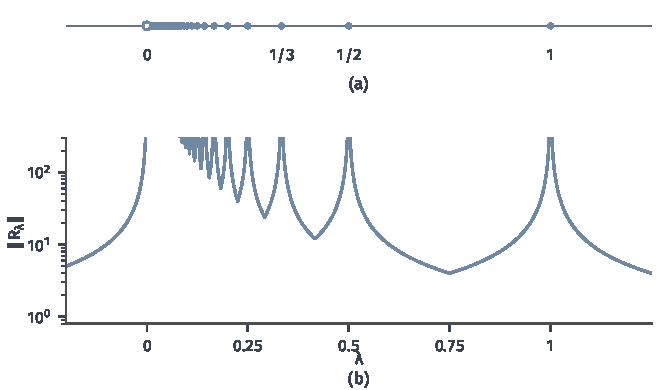
\includegraphics[width=112mm]{figures/04-spaces-measures-and-geometry/03-function-spaces/matplotlib/ospec-spectrum-resolvent/figure.pdf}
  \caption{$\ell^2$上$A(x_n)=(x_n/n)$的谱。(a)~特征值$1/n$（实心点）向$0$聚集，$0$属于谱但不是特征值（空心点）。(b)~实参数$\lambda$处预解算子的范数，纵轴取对数；各谱点处的尖峰向$0$聚集，靠近$0$时尖峰之间的低谷也越出了纵轴范围。}
  \label{fig:ospec-spectrum-resolvent}
\end{BookInlineFigure}

\paragraph{累积积分没有特征值}
紧性保证了非零谱点的有限维结构，却不保证有足够多的特征向量。在$L^2(0,1)$上令
\[
(Vf)(x)=\int_0^xf(t)\,\mathrm dt.
\]
它的核$\mathbf 1_{\{t<x\}}$平方可积，由第~\ref{chap:linear-operators}章，$V$是紧算子。

设$Vf=\lambda f$，$\lambda\neq0$。右端$Vf$连续，所以$f=\lambda^{-1}Vf$连续；于是$Vf$连续可导，$f$也连续可导。对$Vf=\lambda f$求导，并在$x=0$处取值，得到
\[
\lambda f^\prime=f,\qquad f(0)=\lambda^{-1}(Vf)(0)=0.
\]
这个初值问题的解是$f(x)=f(0)\mathrm e^{x/\lambda}=0$，所以$V$没有非零特征值。

$\lambda=0$也不是特征值。$Vf=0$说明$f$在每个区间$[0,x]$上积分为零，相减后在每个区间上积分为零。区间示性函数的线性组合在$L^2(0,1)$中稠密（第~\ref{chap:wavelet-transform}章），$f$与一个稠密集正交，只能为零。

由定理~\ref{thm:ospec-compact-spectrum}，非零谱点都是特征值，因此$\sigma(V)=\{0\}$，而$V$一个特征向量也没有。像的情况也可以判定：$V^*g(t)=\int_t^1g$，同样的论证给出$\ker V^*=\{0\}$，所以$V$的像稠密，$0$属于连续谱。

离散化可以看出这件事的矩阵对应物。把$[0,1]$分成$n$段，取$h=1/n$，累积积分变成$(\bm V_n\bm x)_i=h\sum_{j\leq i}x_j$，它是下三角矩阵，对角元全是$h$。特征值只有$h$，随$n$增大趋于$0$，与$\sigma(V)=\{0\}$相符；而$\bm V_n-h\bm I$的秩是$n-1$，整个矩阵只有一个特征方向。特征方向的严重不足，到了无限维就成了一个也没有。

\paragraph{五个例子的比较}
表~\ref{tab:ospec-gallery}汇总了本章到目前为止的算子。前三个不是紧算子，谱可以是区间或圆盘；后两个紧，谱都收缩到可数集，连续谱只剩$\{0\}$。

\begin{table}[!htb]
  \centering
  \caption{五个算子的谱。$M$是$L^2(0,1)$上乘以$x$的算子，$S$与$L$是$\ell^2$上的右移与左移，$A=\operatorname{diag}(1/n)$，$V$是累积积分；$\mathbb D$表示开单位圆盘，$\mathbb T$表示单位圆周。}
  \label{tab:ospec-gallery}
  \begin{tabular}{@{}cllll@{}}
    \toprule
    算子 & 谱 & 点谱 & 连续谱 & 剩余谱\\
    \midrule
    $M$ & $[0,1]$ & $\varnothing$ & $[0,1]$ & $\varnothing$\\
    $S$ & $\overline{\mathbb D}$ & $\varnothing$ & $\mathbb T$ & $\mathbb D$\\
    $L$ & $\overline{\mathbb D}$ & $\mathbb D$ & $\mathbb T$ & $\varnothing$\\
    $A$ & $\{1/n\}\cup\{0\}$ & $\{1/n\}$ & $\{0\}$ & $\varnothing$\\
    $V$ & $\{0\}$ & $\varnothing$ & $\{0\}$ & $\varnothing$\\
    \bottomrule
  \end{tabular}
\end{table}

表中$L$的圆周部分这样判定：$\lvert\lambda\rvert=1$时，特征方程的解$(c,c\lambda,c\lambda^2,\ldots)$不平方可和，所以$L-\lambda I$是单射；由$\ker(S-\bar\lambda I)=\{0\}$，它的像稠密；谱是闭集，圆周属于谱。

两个紧算子的对比划出了本节结论的边界。紧性把非零谱变成离散的特征值，但不保证特征向量张满空间，更不保证它们彼此正交；$V$的谱只有一个点，任何沿特征方向的展开都不存在。下一节加入自伴条件，正是为了得到正交而完备的特征方向。

\section{紧自伴算子的谱分解}
\label{sec:ospec-compact-self-adjoint}

实对称矩阵有一组由特征向量组成的标准正交基，矩阵在这组基下是实对角矩阵。上一节的累积积分说明，紧性本身不足以给出这种结构；对角算子$A(x_n)=(x_n/n)$却正好具备它：特征向量$e_n$组成标准正交基，算子就是沿每个基方向乘以一个数。二者的差别在于$A$是自伴的。本节证明，在Hilbert空间中对紧算子再加入自伴条件，就得到实特征值、正交的特征方向，以及Hilbert范数下的特征展开。

本节设$H$是实或复Hilbert空间，$T\in\mathcal B(H)$紧且自伴，即$\langle v,Tu\rangle=\langle Tv,u\rangle$对一切$u,v$成立。证明不需要复化：自伴算子的特征值将被证明是实数。

\begin{theorem}[紧自伴算子的谱分解]
\label{thm:ospec-compact-self-adjoint}
设$T$是Hilbert空间$H$上的紧自伴算子。则：
\begin{enumerate}
\item $T$的特征值都是实数，属于不同特征值的特征向量互相正交；
\item 每个非零特征值的特征空间有限维；对每个$\delta>0$，满足$\lvert\lambda\rvert\geq\delta$的特征值只有有限个；
\item 存在有限或可数的标准正交序列$(e_j)$及非零实数$\lambda_j$（按重数重复列出，$\lvert\lambda_1\rvert\geq\lvert\lambda_2\rvert\geq\cdots$，序列无限时$\lambda_j\to0$），使$Te_j=\lambda_je_j$，$(e_j)$的闭张成等于$(\ker T)^\perp$，并且对每个$u\in H$，
\begin{equation}
u=u_0+\sum_j\langle e_j,u\rangle e_j,\qquad Tu=\sum_j\lambda_j\langle e_j,u\rangle e_j,\qquad u_0\in\ker T,
\label{eq:ospec-spectral-expansion}
\end{equation}
两个级数都按$H$的范数收敛。
\end{enumerate}
\end{theorem}

证明的主线是：先说明自伴算子的范数可以由二次型$\langle u,Tu\rangle$读出，再用紧性找到使二次型绝对值最大的方向，它就是一个特征方向；然后把算子限制到这个方向的正交补上，重复同样的步骤。下面分步完成。

\paragraph{特征值与正交性}
设$Tu=\lambda u$，$u\neq0$。由内积对第一个变量共轭线性，$\langle u,Tu\rangle=\lambda\lVert u\rVert^2$，$\langle Tu,u\rangle=\bar\lambda\lVert u\rVert^2$；自伴使两者相等，所以$\lambda=\bar\lambda$是实数。再设$Tv=\mu v$，$\mu\neq\lambda$，两者都是实数，于是
\[
\lambda\langle v,u\rangle=\langle v,Tu\rangle=\langle Tv,u\rangle=\mu\langle v,u\rangle ,
\]
从而$\langle v,u\rangle=0$。这证明了结论1。

\paragraph{非零特征值的有限性}
设$(e_j)$是一列两两正交的单位特征向量，$Te_j=\lambda_je_j$且$\lvert\lambda_j\rvert\geq\delta>0$；它们可以来自同一个特征空间的标准正交组，也可以属于不同特征值（由结论1自动正交）。对$j\neq k$，
\[
\lVert Te_j-Te_k\rVert^2=\lVert\lambda_je_j-\lambda_ke_k\rVert^2=\lvert\lambda_j\rvert^2+\lvert\lambda_k\rvert^2\geq2\delta^2 ,
\]
输出列没有柯西子列，与紧性矛盾，所以这种序列只能有限长。取同一特征空间中的标准正交组，即知非零特征空间有限维；取不同特征值的特征向量，即知$\lvert\lambda\rvert\geq\delta$的特征值只有有限个。这证明了结论2，它在Hilbert空间中重现了上一节定理的相应部分，而且证明更短，因为正交性代替了Riesz引理。

\paragraph{二次型给出范数}
令$M=\sup_{\lVert u\rVert=1}\lvert\langle u,Tu\rangle\rvert$。由Cauchy--Schwarz不等式$M\leq\lVert T\rVert$。反向不等式要从二次型恢复$\lVert Tu\rVert$。自伴使$\langle u,Tv\rangle=\langle Tu,v\rangle=\overline{\langle v,Tu\rangle}$，展开可得
\[
\langle u+v,T(u+v)\rangle-\langle u-v,T(u-v)\rangle=2\langle u,Tv\rangle+2\langle v,Tu\rangle=4\operatorname{Re}\langle v,Tu\rangle .
\]
左边两项的绝对值分别不超过$M\lVert u+v\rVert^2$与$M\lVert u-v\rVert^2$，再用平行四边形恒等式$\lVert u+v\rVert^2+\lVert u-v\rVert^2=2\lVert u\rVert^2+2\lVert v\rVert^2$，得
\[
4\operatorname{Re}\langle v,Tu\rangle\leq2M\bigl(\lVert u\rVert^2+\lVert v\rVert^2\bigr).
\]
对单位向量$u$且$Tu\neq0$，取$v=Tu/\lVert Tu\rVert$，则$\operatorname{Re}\langle v,Tu\rangle=\lVert Tu\rVert$，上式化为$\lVert Tu\rVert\leq M$。因此$\lVert T\rVert=M$。

\paragraph{紧性给出极值方向}
设$T\neq0$。取单位向量$u_n$使$\lvert\langle u_n,Tu_n\rangle\rvert\to\lVert T\rVert$。这些二次型都是实数，可以抽出子列使它们的符号一致，于是$\langle u_n,Tu_n\rangle\to\lambda$，其中$\lambda=\lVert T\rVert$或$-\lVert T\rVert$。这里不能预先假定$\lambda$为正：自伴算子的二次型可以取负值，绝对值最大的特征值可能是负的。展开
\[
\lVert Tu_n-\lambda u_n\rVert^2=\lVert Tu_n\rVert^2-2\lambda\langle u_n,Tu_n\rangle+\lambda^2\leq2\lambda^2-2\lambda\langle u_n,Tu_n\rangle\to0 ,
\]
其中用到$\lVert Tu_n\rVert\leq\lVert T\rVert=\lvert\lambda\rvert$。

由紧性，可再抽子列使$Tu_n\to w$。于是$\lambda u_n=Tu_n-(Tu_n-\lambda u_n)\to w$，即$u_n\to e=w/\lambda$，$\lVert e\rVert=1$，并且$Te=\lim Tu_n=w=\lambda e$。所以$\pm\lVert T\rVert$中至少有一个是特征值，相应单位特征向量为$e$。

\paragraph{逐步分解与零空间}
记$e_1=e$，$\lambda_1=\lambda$。正交补$H_2=\{e_1\}^\perp$在$T$下不变：若$\langle e_1,v\rangle=0$，则$\langle e_1,Tv\rangle=\langle Te_1,v\rangle=\lambda_1\langle e_1,v\rangle=0$。$T$在$H_2$上的限制仍是紧自伴算子，范数不超过$\lVert T\rVert$。若这个限制为零，过程停止；否则重复上一段，得到$e_2\perp e_1$及$\lvert\lambda_2\rvert=\lVert T|_{H_2}\rVert\leq\lvert\lambda_1\rvert$。依此类推，在$H_k=\{e_1,\ldots,e_{k-1}\}^\perp$上取$e_k$。若过程不停止，由结论2，$\lambda_k\to0$。

令$M$为$(e_j)$的闭张成。$M^\perp$含于每个$H_k$，所以$T$在$M^\perp$上的限制的范数不超过每个$\lvert\lambda_k\rvert$；过程无限时它趋于零，有限时按停止条件本身为零。因此$T$在$M^\perp$上恒为零，$M^\perp\subseteq\ker T$。反过来，若$Tu=0$，则对每个$j$，
\[
\langle e_j,u\rangle=\frac{1}{\lambda_j}\langle Te_j,u\rangle=\frac{1}{\lambda_j}\langle e_j,Tu\rangle=0 ,
\]
所以$\ker T\subseteq M^\perp$。二者相等，$M=(M^\perp)^\perp=(\ker T)^\perp$。这也说明每个非零特征值都已出现在$(\lambda_j)$中：属于非零特征值$\mu$的特征向量与$\ker T$正交，因而落在$M$中；若$\mu$不等于任何$\lambda_j$，由结论1它与所有$e_j$正交，只能为零。

\paragraph{展开式}
$u$在闭子空间$M$上的正交投影为$\sum_j\langle e_j,u\rangle e_j$，级数按范数收敛（第~\ref{chap:inner-product-spaces}章）；余项$u_0=u-P_Mu$属于$M^\perp=\ker T$。把$T$作用于投影的部分和，由连续性得$Tu=\sum_j\lambda_j\langle e_j,u\rangle e_j$。这就是式\eqref{eq:ospec-spectral-expansion}，定理证毕。

\paragraph{空间的分解与有限谱截断}
定理把$H$分成两部分：$\ker T$与非零特征方向的闭张成$(\ker T)^\perp$。任意向量$u$的位置由它在$\ker T$中的分量$u_0$与各特征方向上的系数$\langle e_j,u\rangle$完全确定，$T$消去$u_0$，并把第$j$个系数乘以$\lambda_j$。由勾股定理，
\[
\lVert u\rVert^2=\lVert u_0\rVert^2+\sum_j\lvert\langle e_j,u\rangle\rvert^2,\qquad\lVert Tu\rVert^2=\sum_j\lambda_j^2\lvert\langle e_j,u\rangle\rvert^2 .
\]

只保留前$m$个特征方向，得到有限秩算子$T_mu=\sum_{j\leq m}\lambda_j\langle e_j,u\rangle e_j$。由上式，
\[
\lVert(T-T_m)u\rVert^2=\sum_{j>m}\lambda_j^2\lvert\langle e_j,u\rangle\rvert^2\leq\lambda_{m+1}^2\lVert u\rVert^2 ,
\]
取$u=e_{m+1}$时等号成立，所以$\lVert T-T_m\rVert=\lvert\lambda_{m+1}\rvert$（非零特征值用尽时约定为$0$）。特征值按绝对值递减排列，截断误差就是第一个被舍弃的特征值的绝对值；这给出第~\ref{chap:linear-operators}章有限秩逼近的一个具体而经济的选择。

\paragraph{贯穿例子}
回到$L^2([-1,1],\mu)$，$\mathrm d\mu=\mathrm dz/2$，核$1+xz$给出$(Tf)(x)=\int f\,\mathrm d\mu+x\int zf\,\mathrm d\mu$。核实对称，$T$紧自伴。由$T1=1$与$Tx=x\int z^2\,\mathrm d\mu=\tfrac13x$，单位特征向量为$e_1=1$、$e_2=\sqrt3\,x$，特征值$\lambda_1=1$、$\lambda_2=1/3$，于是
\[
Tf=\langle e_1,f\rangle e_1+\tfrac13\langle e_2,f\rangle e_2 .
\]
与$1,x$都正交的函数组成$\ker T$，例如$x^2-1/3$，这个零空间是无限维的。截断一项的误差为$\lVert T-T_1\rVert=1/3$。

把核换成$1-6xz$，常数方向不变，线性方向变为$Tx=-6x\int z^2\,\mathrm d\mu=-2x$，绝对值最大的特征值是$-2$。若只寻找正的最大特征值，就会漏掉这个主导方向，这正是证明中不预设$\lambda>0$的原因。图~\ref{fig:ospec-spectral-stretch}在两组特征方向的系数平面上画出了这两类伸缩。

\begin{figure}[!htb]
  \centering
  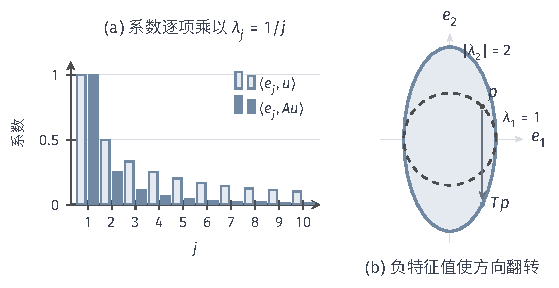
\includegraphics[width=94.6mm]{figures/02-abstract-mathematics/03-function-spaces/tikz/c3-spectral-stretch/figure.pdf}
  \caption{紧自伴算子沿特征方向逐个伸缩。(a)~$\ell^2$上$A=\operatorname{diag}(1/j)$，浅色条为$u$的系数$\langle e_j,u\rangle=1/j$，深色条为$Au$的系数$1/j^2$；(b)~$L^2([-1,1],\mathrm dz/2)$上核$1-6xz$的积分算子，在$e_1=1$、$e_2=\sqrt3x$的系数平面上把虚线单位圆映为实线椭圆：$e_1$方向乘$1$，$e_2$方向乘$-2$。与$1,x$正交的方向全部被映为零，图中未画出。}
  \label{fig:ospec-spectral-stretch}
\end{figure}

谱分解中的级数按Hilbert空间的范数收敛。对$L^2$中的函数，这意味着平方积分误差趋于零，并不意味着在每一点或一致地收敛；第~\ref{sec:ospec-integral-expansion}节在积分核上具体讨论这一区别。

\section{紧算子的奇异分解}
\label{sec:ospec-singular}

累积积分$V$没有特征向量，从$L^2(\nu)$到另一个空间$L^2(\mu)$的积分算子更谈不上$T-\lambda I$。有限维中，矩阵的奇异值分解用输入、输出各一组标准正交方向解决这个问题，可参考\BookChapterRef{chap:singular-value-decomposition}{卷二第5章“奇异值分解”}。对紧算子，同样的构造可以通过正的紧自伴算子$T^*T$完成，而不要求原算子自伴，也不要求输入与输出位于同一空间。

本节设$H_1,H_2$是Hilbert空间，$T:H_1\to H_2$是紧算子。

\paragraph{从$T^*T$构造两组方向}
$T^*T:H_1\to H_1$是紧算子，因为它是有界算子$T^*$与紧算子$T$的复合；它自伴，并且
\[
\langle x,T^*Tx\rangle=\langle Tx,Tx\rangle=\lVert Tx\rVert^2\geq0 ,
\]
所以是正算子，特征值都非负，并且$T^*Tx=0$当且仅当$Tx=0$，即$\ker(T^*T)=\ker T$。

对$T^*T$应用定理~\ref{thm:ospec-compact-self-adjoint}，得到标准正交的特征向量$v_j$与正特征值$s_j$，按递减顺序排列。令$\sigma_j=\sqrt{s_j}$，再令$u_j=Tv_j/\sigma_j$。这组输出方向也标准正交：
\[
\langle u_j,u_k\rangle=\frac{\langle Tv_j,Tv_k\rangle}{\sigma_j\sigma_k}=\frac{\langle v_j,T^*Tv_k\rangle}{\sigma_j\sigma_k}=\frac{\sigma_k^2\langle v_j,v_k\rangle}{\sigma_j\sigma_k}=\delta_{j,k} .
\]
此外$T^*u_j=T^*Tv_j/\sigma_j=\sigma_jv_j$，所以$T$把$v_j$送到$\sigma_ju_j$，$T^*$把$u_j$送回$\sigma_jv_j$。

\begin{theorem}[紧算子的奇异分解]
\label{thm:ospec-svd}
设$T:H_1\to H_2$是紧算子，$\sigma_1\geq\sigma_2\geq\cdots>0$及标准正交序列$(v_j)\subseteq H_1$、$(u_j)\subseteq H_2$如上构造。则对每个$x\in H_1$、$y\in H_2$，
\begin{equation}
Tx=\sum_j\sigma_j\langle v_j,x\rangle u_j,\qquad T^*y=\sum_j\sigma_j\langle u_j,y\rangle v_j ,
\label{eq:ospec-svd}
\end{equation}
级数按范数收敛。$(v_j)$的闭张成为$(\ker T)^\perp$，$(u_j)$的闭张成为$\overline{\operatorname{Ran}T}=(\ker T^*)^\perp$。序列无限时$\sigma_j\to0$。
\end{theorem}

\begin{proof}
由定理~\ref{thm:ospec-compact-self-adjoint}，$(v_j)$的闭张成为$(\ker T^*T)^\perp=(\ker T)^\perp$，任意$x$可写成$x=x_0+\sum_j\langle v_j,x\rangle v_j$，$x_0\in\ker T$。把$T$作用于部分和并取极限，得$Tx=\sum_j\langle v_j,x\rangle Tv_j=\sum_j\sigma_j\langle v_j,x\rangle u_j$。

由这一展开，每个$Tx$都落在$(u_j)$的闭张成中；反之每个$u_j=T(v_j/\sigma_j)$属于$\operatorname{Ran}T$。所以$(u_j)$的闭张成等于$\overline{\operatorname{Ran}T}$，再由第~\ref{chap:linear-operators}章的正交关系，它等于$(\ker T^*)^\perp$。

关于$T^*$的展开，对任意$x$有
\[
\langle x,T^*y\rangle=\langle Tx,y\rangle=\sum_j\sigma_j\overline{\langle v_j,x\rangle}\langle u_j,y\rangle=\Bigl\langle x,\sum_j\sigma_j\langle u_j,y\rangle v_j\Bigr\rangle ,
\]
右端级数因系数平方可和而收敛，两边对一切$x$相等，故展开成立。$\sigma_j\to0$来自$s_j\to0$。
\end{proof}

数$\sigma_j$称为$T$的\term{奇异值}（singular value），$v_j$与$u_j$分别称为\term{右奇异向量}（right singular vector）与\term{左奇异向量}（left singular vector），三者合称$T$的\term{奇异系统}（singular system）。函数空间中，左右奇异向量也称左右奇异函数。

展开式\eqref{eq:ospec-svd}把$T$的作用拆成三步：读出输入在$v_j$方向上的系数，乘以$\sigma_j$，再放到输出方向$u_j$上。输入空间分成$\ker T$与$\overline{\operatorname{span}}\{v_j\}$，前者的分量在输出中完全看不见；输出空间分成$\ker T^*$与$\overline{\operatorname{span}}\{u_j\}$，前者是任何输入都到达不了的方向。两组方向一般位于不同的空间；即使$H_1=H_2$，$u_j$也未必等于$v_j$。对正的紧自伴算子，两组方向可以取得相同，奇异值就是特征值；对一般自伴算子，奇异值是特征值的绝对值，负特征值的方向上$u_j=-v_j$。

\begin{example}[累积积分的奇异分解]
\label{ex:ospec-volterra-svd}
在$L^2(0,1)$上，$(Vf)(x)=\int_0^xf(t)\,\mathrm dt$是紧算子，伴随为$(V^*g)(t)=\int_t^1g(x)\,\mathrm dx$（第~\ref{chap:linear-operators}章），于是
\[
(V^*Vf)(t)=\int_t^1\Bigl(\int_0^xf(s)\,\mathrm ds\Bigr)\mathrm dx .
\]

设$V^*Vf=sf$，$s>0$。右端是连续函数，所以$f=s^{-1}V^*Vf$连续；于是$Vf$连续可导，$V^*Vf$二次连续可导，$f$也二次连续可导。对$t$求导两次得$(V^*Vf)^\prime=-Vf$、$(V^*Vf)^{\prime\prime}=-f$，因此$sf^{\prime\prime}=-f$；又由表达式直接读出$(V^*Vf)^\prime(0)=0$、$(V^*Vf)(1)=0$，故$f^\prime(0)=0$、$f(1)=0$。满足这些条件的非零解为$f(t)=c\cos(\omega t)$，其中$\omega=s^{-1/2}$且$\cos\omega=0$，即$\omega_k=(k-\tfrac12)\pi$，$k=1,2,\ldots$。

上一节已证明$V$是单射，所以$\ker V^*V=\ker V=\{0\}$，$V^*V$的特征向量张满整个$L^2(0,1)$。由此
\begin{equation*}
\begin{gathered}
\sigma_k=\frac{1}{(k-\frac12)\pi}=\frac{2}{(2k-1)\pi},\\
v_k(t)=\sqrt2\cos\bigl((k-\tfrac12)\pi t\bigr),\qquad u_k(x)=\sqrt2\sin\bigl((k-\tfrac12)\pi x\bigr),
\end{gathered}
\end{equation*}
其中$u_k=Vv_k/\sigma_k$可直接积分验证，归一化由$\int_0^12\cos^2(\omega_kt)\,\mathrm dt=1+\sin(2\omega_k)/(2\omega_k)=1$核对。前几个奇异值约为$0.637$、$0.212$、$0.127$、$0.091$，按$1/k$的速度衰减。
\end{example}

$V$没有特征向量，却有完整的奇异系统：输入方向是余弦族，输出方向是正弦族，两组方向不同。这说明奇异分解确实不依赖自伴性，它对每个紧算子都存在。

\paragraph{截断奇异分解}
只保留前$m$项，得到秩不超过$m$的算子
\[
T_mx=\sum_{j\leq m}\sigma_j\langle v_j,x\rangle u_j .
\]
下面的定理说明，截断误差恰为第一个被舍弃的奇异值，并且没有任何秩不超过$m$的算子能做得更好。正奇异值只有有限个时，约定用尽之后的$\sigma_j=0$。

\begin{theorem}[截断奇异分解的误差]
\label{thm:ospec-svd-truncation}
在定理~\ref{thm:ospec-svd}的条件下，$\lVert T-T_m\rVert=\sigma_{m+1}$；并且对每个秩不超过$m$的有界算子$F:H_1\to H_2$，都有$\lVert T-F\rVert\geq\sigma_{m+1}$。
\end{theorem}

\begin{proof}
第一步，计算截断误差。由式\eqref{eq:ospec-svd}及$(u_j)$的正交性，
\[
\lVert(T-T_m)x\rVert^2=\sum_{j>m}\sigma_j^2\lvert\langle v_j,x\rangle\rvert^2\leq\sigma_{m+1}^2\sum_{j>m}\lvert\langle v_j,x\rangle\rvert^2\leq\sigma_{m+1}^2\lVert x\rVert^2 ,
\]
最后一步是Bessel不等式。若$\sigma_{m+1}>0$，取$x=v_{m+1}$时等号成立，所以$\lVert T-T_m\rVert=\sigma_{m+1}$。

第二步，证明下界。不妨设$\sigma_{m+1}>0$。令$W=\operatorname{span}\{v_1,\ldots,v_{m+1}\}$，它是$m+1$维的。$F$把$W$映入维数不超过$m$的$\operatorname{Ran}F$，由维数公式，存在单位向量$x\in W$使$Fx=0$。写$x=\sum_{j\leq m+1}c_jv_j$，$\sum_j\lvert c_j\rvert^2=1$，则
\[
\lVert(T-F)x\rVert^2=\lVert Tx\rVert^2=\sum_{j\leq m+1}\sigma_j^2\lvert c_j\rvert^2\geq\sigma_{m+1}^2 .
\]
因此$\lVert T-F\rVert\geq\sigma_{m+1}$。
\end{proof}

图~\ref{fig:ospec-svd-decay}在累积积分上展示这一结论。保留前三项时误差为$\sigma_4\approx0.091$；奇异值衰减越快，同样秩的截断误差越小。奇异值越小的方向振荡越快：$V$是积分，它把快速振荡的输入平均掉，输出的幅度只剩$1/\omega_k$倍。对比$\ell^2$上的$A(x_n)=(x_n/n)$，它是正自伴算子，奇异值就是特征值$1/n$，左右奇异向量都是$e_n$，第~\ref{chap:linear-operators}章对它的坐标截断正是截断奇异分解。

\begin{figure}[!htb]
  \centering
  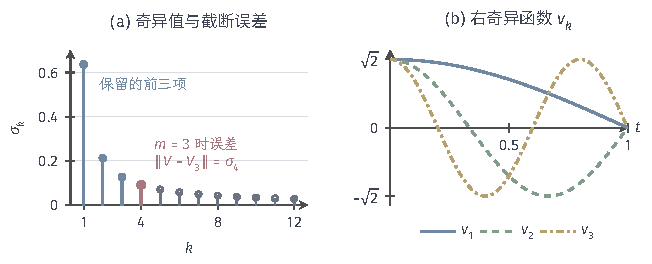
\includegraphics[width=110.3mm]{figures/02-abstract-mathematics/03-function-spaces/tikz/c3-svd-decay/figure.pdf}
  \caption{累积积分$(Vf)(x)=\int_0^xf$在$L^2(0,1)$上的奇异分解。(a)~奇异值$\sigma_k=2/((2k-1)\pi)$；保留前三项（蓝色）时，算子范数误差等于第四个奇异值$\sigma_4\approx0.091$（红色），后面的奇异值（空心）全部被舍去；(b)~前三个右奇异函数$v_k(t)=\sqrt2\cos((k-\frac12)\pi t)$，序号越大振荡越快。}
  \label{fig:ospec-svd-decay}
\end{figure}

小奇异值对正向逼近是好消息：舍去它们，误差很小。对反向求解却是坏消息：从输出恢复输入，要把这些方向上的系数除以$\sigma_j$。这一障碍是第~\ref{chap:linear-operator-equations}章讨论第一类方程时的核心问题。

\section{积分算子的谱展开}
\label{sec:ospec-integral-expansion}

第~\ref{chap:linear-operators}章证明了：$\sigma$有限测度空间上的平方可积核给出有界的紧积分算子，伴随的核是原核交换变量后取共轭，核的$L^2$误差控制算子范数误差。本节把前几节的展开落实到这些核上。算子的展开是关于输入函数$f$的级数；核是乘积空间上的一个函数，它也可以展开成乘积函数的级数。两种展开所用的收敛意义不同，这是本节要分清的主要问题。

下面设$(X,\mu)$、$(Y,\nu)$是$\sigma$有限测度空间，$k\in L^2(X\times Y,\mu\otimes\nu)$，$T:L^2(Y,\nu)\to L^2(X,\mu)$是以$k$为核的积分算子。对$a\in L^2(\mu)$、$b\in L^2(\nu)$，记$(a\otimes\bar b)(x,y)=a(x)\overline{b(y)}$。先建立两个把“核”与“算子”联系起来的工具。

\begin{lemma}[乘积函数与核系数]
\label{lem:ospec-product-coefficients}
设$(a_j)\subseteq L^2(\mu)$、$(b_l)\subseteq L^2(\nu)$都是标准正交序列。则$\{a_j\otimes\bar b_l\}$是$L^2(\mu\otimes\nu)$中的标准正交族，并且
\[
\langle a_j\otimes\bar b_l,k\rangle_{L^2(\mu\otimes\nu)}=\langle a_j,Tb_l\rangle_{L^2(\mu)} .
\]
\end{lemma}

\begin{proof}
函数$\lvert a_j(x)\rvert^2\lvert b_l(y)\rvert^2$的积分由Tonelli定理等于$\lVert a_j\rVert^2\lVert b_l\rVert^2=1$，所以$a_j\otimes\bar b_l\in L^2(\mu\otimes\nu)$。两个乘积函数之积可积（Cauchy--Schwarz），由Fubini定理分离变量，
\begin{equation*}
\begin{aligned}
\langle a_j\otimes\bar b_l,a_{j^\prime}\otimes\bar b_{l^\prime}\rangle&=\int\overline{a_j}a_{j^\prime}\,\mathrm d\mu\cdot\int b_l\overline{b_{l^\prime}}\,\mathrm d\nu\\
&=\langle a_j,a_{j^\prime}\rangle\,\langle b_{l^\prime},b_l\rangle=\delta_{j,j^\prime}\delta_{l,l^\prime}.
\end{aligned}
\end{equation*}
同样，$\overline{a_j(x)}b_l(y)k(x,y)$在乘积空间上可积，先对$y$积分得
\begin{equation*}
\int_X\overline{a_j(x)}(Tb_l)(x)\,\mathrm d\mu(x)=\langle a_j,Tb_l\rangle.
\end{equation*}
\end{proof}

\begin{lemma}[核由算子唯一确定]
\label{lem:ospec-kernel-unique}
若$r\in L^2(\mu\otimes\nu)$给出的积分算子为零，则$r=0$在$\mu\otimes\nu$几乎处处成立。
\end{lemma}

\begin{proof}
对$\mu(A)<\infty$、$\nu(B)<\infty$，有$\langle\mathbf 1_A\otimes\mathbf 1_B,r\rangle=\langle\mathbf 1_A,T_r\mathbf 1_B\rangle=0$，计算方式同上一引理。第~\ref{chap:linear-operators}章证明了这类矩形示性函数的线性组合在$L^2(\mu\otimes\nu)$中稠密，所以$r$与一个稠密集正交，只能为零。
\end{proof}

\subsection{自伴积分算子的特征展开}
\label{sec:ospec-self-adjoint-kernel}

取$X=Y$、$\mu=\nu$，并设$k(x,y)=\overline{k(y,x)}$对$\mu\otimes\mu$几乎处处成立。由第~\ref{chap:linear-operators}章，$T$是$L^2(\mu)$上的紧自伴算子，定理~\ref{thm:ospec-compact-self-adjoint}给出标准正交特征函数$(e_j)$与非零实特征值$(\lambda_j)$。

\begin{theorem}[自伴积分算子的特征展开]
\label{thm:ospec-self-adjoint-kernel}
在上述条件下，
\begin{enumerate}
\item 对每个$f\in L^2(\mu)$，$Tf=\sum_j\lambda_j\langle e_j,f\rangle e_j$，级数在$L^2(\mu)$中收敛；
\item 核满足$k=\sum_j\lambda_j\,e_j\otimes\bar e_j$，即$k(x,y)=\sum_j\lambda_je_j(x)\overline{e_j(y)}$，级数在$L^2(\mu\otimes\mu)$中收敛；
\item $\lVert k\rVert_{L^2(\mu\otimes\mu)}^2=\sum_j\lambda_j^2$，截去$j>m$各项后核的$L^2$误差为$\bigl(\sum_{j>m}\lambda_j^2\bigr)^{1/2}$。
\end{enumerate}
\end{theorem}

\begin{proof}
（1）就是式\eqref{eq:ospec-spectral-expansion}。（2）由引理~\ref{lem:ospec-product-coefficients}，$k$关于标准正交族$\{e_j\otimes\bar e_l\}$的系数为$\langle e_j,Te_l\rangle=\lambda_l\delta_{j,l}$。由Bessel不等式$\sum_j\lambda_j^2\leq\lVert k\rVert^2<\infty$，所以$\tilde k=\sum_j\lambda_je_j\otimes\bar e_j$在$L^2(\mu\otimes\mu)$中收敛。

记$k_m$为前$m$项的部分和，它给出算子$T_{k_m}f=\sum_{j\leq m}\lambda_j\langle e_j,f\rangle e_j$。由核误差控制算子误差，$T_{k_m}\to T_{\tilde k}$按算子范数收敛；由（1），$T_{k_m}f\to Tf$对每个$f$成立。所以$T_{\tilde k}=T$，核$k-\tilde k$给出零算子，由引理~\ref{lem:ospec-kernel-unique}，$k=\tilde k$几乎处处。

（3）由正交展开的勾股定理，$\lVert k\rVert^2=\lVert\tilde k\rVert^2=\sum_j\lambda_j^2$，尾部的范数平方为$\sum_{j>m}\lambda_j^2$。
\end{proof}

定理的第（3）条与上一节的截断误差合在一起，给出同一个截断的两种误差：算子范数误差$\lVert T-T_m\rVert=\lvert\lambda_{m+1}\rvert$只看第一个被舍弃的特征值，核的$L^2$误差$(\sum_{j>m}\lambda_j^2)^{1/2}$要把全部舍弃项的平方加起来，后者总不小于前者。

贯穿例子中，$1+xz=1\cdot1+\tfrac13(\sqrt3x)(\sqrt3z)$正是两项的特征展开，$\lVert k\rVert^2=10/9=1^2+(1/3)^2$。第~\ref{chap:linear-operators}章用乘积积分直接算出的$10/9$在这里得到了解释：它是特征值的平方和。截去第二项，核误差与算子误差都等于$1/3$，因为只舍弃了一项。

\paragraph{收敛意义的边界}
核的展开在$L^2(\mu\otimes\mu)$中收敛，意思是$\iint\lvert k-k_m\rvert^2\to0$。它不推出$k_m(x,y)\to k(x,y)$对每一对$(x,y)$成立，更不推出一致收敛。这不只是技术细节：平方可积核本身只是几乎处处的等价类，在零测集上改动它不改变积分算子。例如在$[-1,1]^2$上令$k^\prime(x,z)=1+xz-10\cdot\mathbf 1_{\{x=z\}}$，对角线在乘积测度下为零测集，$k^\prime$与$k$给出同一个正算子，但$k^\prime(x,x)=x^2-9<0$。所以从本节的结论出发，不能谈论核在对角线上的取值，也不能断言展开在每一点成立。

逐点或一致收敛需要附加条件，例如核连续、算子为正，并在紧区域上考虑连续的特征函数代表；这类结论属于第~\ref{chap:rkhs}章的Mercer定理，不由这里的谱分解自动得到。

\subsection{非自伴积分算子的特征展开}
\label{sec:ospec-non-self-adjoint-kernel}

自伴条件要求核关于对角线共轭对称，很多核不满足它。上一节的累积积分说明，一般非自伴紧算子可能连一个特征向量都没有，更没有完备的特征系统。本小节先给出一类仍有正交特征展开的非自伴算子，再说明其余情形改用奇异分解。

\paragraph{正规算子}
设$H$是复Hilbert空间。若$T\in\mathcal B(H)$满足$T^*T=TT^*$，则称$T$为\term{正规算子}（normal operator）。自伴算子显然正规；反自伴算子$T^*=-T$也正规，却不自伴（$T\neq0$时）。对积分算子，由伴随核公式，$T^*T$与$TT^*$的核分别是$\int\overline{k(z,x)}k(z,y)\,\mathrm d\mu(z)$与$\int k(x,z)\overline{k(y,z)}\,\mathrm d\mu(z)$，正规条件就是这两个核几乎处处相等。

\begin{theorem}[紧正规算子的谱分解]
\label{thm:ospec-compact-normal}
设$T$是复Hilbert空间$H$上的紧正规算子。则存在有限或可数的标准正交序列$(e_j)$及非零复数$\mu_j$（序列无限时$\mu_j\to0$），使$Te_j=\mu_je_j$，$(e_j)$的闭张成等于$(\ker T)^\perp$，并且$Tu=\sum_j\mu_j\langle e_j,u\rangle e_j$对每个$u\in H$成立。
\end{theorem}

\begin{proof}
令$A=(T+T^*)/2$、$B=(T-T^*)/(2\mathrm i)$。二者都是紧自伴算子，$T=A+\mathrm iB$，并且正规条件推出$AB=BA$。由$T^*T=(A-\mathrm iB)(A+\mathrm iB)=A^2+B^2$，得$\lVert Tu\rVert^2=\lVert Au\rVert^2+\lVert Bu\rVert^2$，所以$\ker T=\ker A\cap\ker B$。

对$A$的每个非零特征值$\alpha$，特征空间$E_\alpha$有限维，并且在$B$下不变：若$Au=\alpha u$，则$A(Bu)=BAu=\alpha Bu$。$B$在$E_\alpha$上的限制是有限维自伴变换，可以取$E_\alpha$的标准正交基使它对角化；这些基向量同时是$A$与$B$的特征向量，因而是$T$的特征向量。同理，$\ker A$在$B$下不变，$B$在$\ker A$上的限制是紧自伴算子，由定理~\ref{thm:ospec-compact-self-adjoint}，它的非零特征方向与零空间$\ker A\cap\ker B$一起张满$\ker A$，这些特征方向上$T=\mathrm iB$。

把两部分的特征向量合在一起，得到标准正交序列$(e_j)$，其闭张成是$\ker T=\ker A\cap\ker B$的正交补，相应特征值$\mu_j=\alpha_j+\mathrm i\beta_j\neq0$。展开式与$\mu_j\to0$的论证与自伴情形相同。
\end{proof}

对平方可积核$k$，若$T$正规，按定理~\ref{thm:ospec-self-adjoint-kernel}同样的证明（引理~\ref{lem:ospec-product-coefficients}给出系数$\langle e_j,Te_l\rangle=\mu_l\delta_{j,l}$），得到核在乘积$L^2$中的正交特征函数展开
\[
k=\sum_j\mu_j\,e_j\otimes\bar e_j,\qquad\lVert k\rVert_{L^2(\mu\otimes\mu)}^2=\sum_j\lvert\mu_j\rvert^2 .
\]

\paragraph{周期卷积核}
在$[0,1)$上取Lebesgue测度，令$h$为$t-\tfrac12$（$t\in[0,1)$）的$1$周期延拓，核$k(x,y)=h(x-y)$。对非整数$t$有$h(-t)=-h(t)$，所以$k(y,x)=-k(x,y)$几乎处处，伴随核为$-k$，$T^*=-T$：$T$正规而不自伴。

特征函数可以直接验证。令$e_n(x)=\mathrm e^{2\pi\mathrm inx}$，$n\in\mathbb Z$。由周期性作变量替换$t=x-y$，
\[
(Te_n)(x)=\int_0^1h(x-y)\mathrm e^{2\pi\mathrm iny}\,\mathrm dy=\mathrm e^{2\pi\mathrm inx}\int_0^1h(t)\mathrm e^{-2\pi\mathrm int}\,\mathrm dt=\mu_ne_n(x).
\]
直接积分得$\mu_0=0$，而$n\neq0$时$\mu_n=\int_0^1t\,\mathrm e^{-2\pi\mathrm int}\,\mathrm dt=\mathrm i/(2\pi n)$。特征值都是纯虚数，这与反自伴相符。

$(e_n)$是$L^2(0,1)$的标准正交基（第~\ref{chap:fourier-transform}章），所以$Tf=\sum_{n\neq0}\mu_n\langle e_n,f\rangle e_n$，$\ker T$由常函数组成。数值核对：$\lVert k\rVert^2=\int_0^1(t-\tfrac12)^2\,\mathrm dt=1/12$，而$\sum_{n\neq0}\lvert\mu_n\rvert^2=2\sum_{n\geq1}\frac{1}{4\pi^2n^2}=\frac{1}{2\pi^2}\cdot\frac{\pi^2}{6}=\frac{1}{12}$，二者相等。

\paragraph{一般核的奇异函数展开}
正规条件不成立时，例如累积积分，或者输入、输出空间根本不同时，回到第~\ref{sec:ospec-singular}节的奇异系统。设$T:L^2(\nu)\to L^2(\mu)$的奇异系统为$(\sigma_j,v_j,u_j)$。

\begin{theorem}[平方可积核的奇异函数展开]
\label{thm:ospec-kernel-svd}
在本节开头的设定下，
\[
k=\sum_j\sigma_j\,u_j\otimes\bar v_j,\qquad\lVert k\rVert_{L^2(\mu\otimes\nu)}^2=\sum_j\sigma_j^2 ,
\]
级数在$L^2(\mu\otimes\nu)$中收敛。记$k_m$为前$m$项之和、$T_m$为相应的截断算子，则
\[
\lVert k-k_m\rVert_{L^2(\mu\otimes\nu)}=\Bigl(\sum_{j>m}\sigma_j^2\Bigr)^{1/2},\qquad\lVert T-T_m\rVert=\sigma_{m+1} .
\]
\end{theorem}

\begin{proof}
由引理~\ref{lem:ospec-product-coefficients}，$k$关于标准正交族$\{u_j\otimes\bar v_l\}$的系数为$\langle u_j,Tv_l\rangle=\sigma_l\langle u_j,u_l\rangle=\sigma_l\delta_{j,l}$。与定理~\ref{thm:ospec-self-adjoint-kernel}的证明相同，Bessel不等式保证级数收敛，部分和给出的算子按算子范数收敛到由式\eqref{eq:ospec-svd}给出的$T$，引理~\ref{lem:ospec-kernel-unique}说明两个核相等。核误差由勾股定理得到，算子误差就是定理~\ref{thm:ospec-svd-truncation}。
\end{proof}

累积积分的核$\mathbf 1_{\{t<x\}}$满足$\lVert k\rVert^2=1/2$，与$\sum_k\sigma_k^2=\frac{4}{\pi^2}\sum_k\frac{1}{(2k-1)^2}=\frac{4}{\pi^2}\cdot\frac{\pi^2}{8}=\frac12$一致。表~\ref{tab:ospec-volterra-errors}列出截断$m$项后的两种误差。

\begin{table}[!htb]
  \centering
  \caption{累积积分截断奇异展开的两种误差。算子范数误差是第一个被舍弃的奇异值$\sigma_{m+1}$，核的$L^2$误差是全部舍弃奇异值平方和的平方根，后者总不小于前者，并且下降得更慢。}
  \label{tab:ospec-volterra-errors}
  \begin{tabular}{@{}ccc@{}}
    \toprule
    保留项数$m$ & 算子误差$\sigma_{m+1}$ & 核误差$(\sum_{j>m}\sigma_j^2)^{1/2}$\\
    \midrule
    $1$ & $0.212$ & $0.308$\\
    $2$ & $0.127$ & $0.223$\\
    $3$ & $0.091$ & $0.183$\\
    $4$ & $0.071$ & $0.159$\\
    \bottomrule
  \end{tabular}
\end{table}

两种误差度量不同的对象。算子误差回答“对最坏的单位输入，近似输出差多少”，它由下一个奇异值决定，按$1/m$下降；核误差回答“作为乘积空间上的函数，近似核差多少”，它累积所有舍去的方向，在这个例子中按$1/\sqrt m$下降。用核误差估计算子误差是安全的上界，却可能过于保守。

\section{本章小结}
\label{sec:ospec-summary}

矩阵的特征值在算子上的对应物是谱，由$T-\lambda I$能否在整个空间上稳定求逆来定义。谱总是有界闭集，含于半径为$\lVert T\rVert$的圆盘，参数越靠近谱，反解的误差放大越严重。有限维中谱只有特征值，无限维多出两类点：连续谱上$T-\lambda I$是单射、像稠密而不满，方程到处可以近似求解，解却不稳定；剩余谱上像不稠密，有一块右端到达不了。

乘法算子把“连续的对角矩阵”这个类比说得最清楚：对角元铺满$[0,1]$，谱是整段区间，却没有特征函数，单位高台只是近似特征向量，极限不在$L^2$中。右移算子的谱是整个闭单位圆盘，内部是剩余谱，边界是连续谱，而它的有限截断只有特征值$0$，说明矩阵截断不一定逼近谱。

紧性使非零谱回到矩阵的情形：非零谱点都是特征值，特征空间有限维，特征值只能向零聚集，单射已经推出可逆。零在无限维中总是谱点，却未必是特征值。累积积分是紧算子，谱只有$\{0\}$，没有一个特征向量，所以紧性本身不保证特征展开。

在Hilbert空间中加入自伴条件，特征值是实数，特征方向两两正交，并与零空间一起张满整个空间，算子作用写成按Hilbert范数收敛的级数，截去前$m$项的算子范数误差是第一个被舍弃的特征值的绝对值。一般紧算子借助$T^*T$得到奇异分解，不要求自伴，也不要求输入输出空间相同，截断误差$\sigma_{m+1}$是秩$m$算子所能达到的最小值。

平方可积核把这些展开变成核函数的展开，核的$L^2$范数对应Frobenius范数，其平方等于特征值或奇异值的平方和；自伴核与正规核有正交特征函数展开，一般核用左右奇异函数展开。同一截断有两种误差：算子误差只看第一个舍弃项，核误差累积全部舍弃项。展开在乘积$L^2$意义下收敛，逐点或一致收敛需要另外的条件。

小奇异值使正向逼近容易、反向恢复困难，这些展开并不自行保证由输出稳定地恢复输入。算子方程的可解条件与稳定性留到第~\ref{chap:linear-operator-equations}章。

